\documentclass{article}
\usepackage[italian]{babel}
\usepackage[T1]{fontenc}
\usepackage{graphicx}
\usepackage[utf8x]{inputenc}
\usepackage{amsmath}
\usepackage{amsthm}
\usepackage{hyperref}
\usepackage{caption}
\date{}
\author{Gruppo 1G.BT \\ Francesco Sacco Lorenzo Cavuoti}
\title{Caratteristiche porte logiche e semplici circuiti logici}

\begin{document}

\maketitle
\paragraph{2)}
	Si è montato il circuito come in figura \ref{fig:d-latch}, e abbiamo ottenuto la tabella di verità \ref{tab:d-latch}, inoltre abbiamo verificato che l'ingresso ENABLE è di predefinito INSERIRE COME è L'INGRESSO DI DEFAULT!\newline
	\begin{minipage}{.6\linewidth}
		\centering
		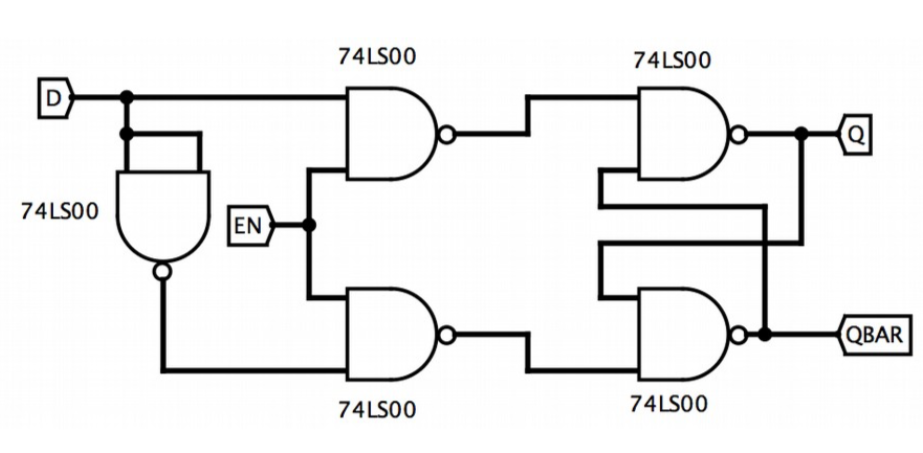
\includegraphics[width=\linewidth]{immagini/dlach}
		\captionof{figure}{Flip-flop D-latch}
		\label{fig:d-latch}
	\end{minipage}
	\begin{minipage}{.4\linewidth}
		\begin{tabular}{cccc}
\hline
	EN & D & Q & !Q\\ 
\hline
	$0$ & X & $Q_{n-1}$ & $!Q_{n-1}$ \\
	$1$ & $0$ & $0$ & $1$ \\
	$1$ & $1$ & $1$ & $0$ \\
\hline
\end{tabular}

		\label{tab:d-latch}
	\end{minipage}\newline
\paragraph{3)}
	Abbiamo montato in divisore in frequenza come nell'immagine \ref{fig:div_freq1} e verificato che il circuito sia effettivamente un contatore da 0 a 15 in codifica binaria.
	In seguito abbiamo inviato un segnale di clock di circa $80 kHz$ e verificato che le uscite dividono il segnale. Qui sotto sono fornite le immagini dell'oscilloscopio.\newline
	\begin{figure}
	\begin{center}
		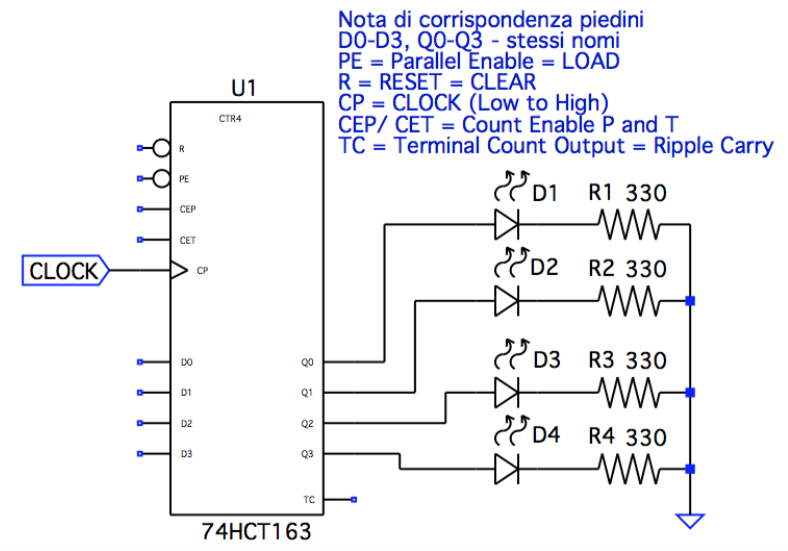
\includegraphics[width=0.5\linewidth]{immagini/div_freq1}
		\captionof{figure}{Schema circuitale del divisore di frequenza}
		\label{fig:div_freq1}
	\end{center}
	\end{figure}
	\newline
	\begin{minipage}{.5\linewidth}
		\centering
		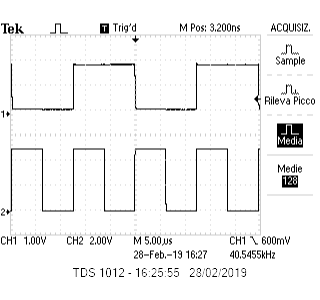
\includegraphics[width=\linewidth]{immagini/f1_2}
		\captionof{figure}{$Q_0$}
		\label{fig:f1_2}
	\end{minipage}
	\begin{minipage}{.5\linewidth}
		\centering
		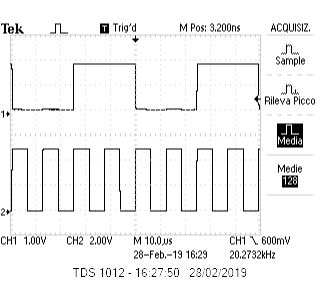
\includegraphics[width=\linewidth]{immagini/f1_4}
		\captionof{figure}{$Q_1$}
		\label{fig:f1_4}
	\end{minipage}\newline
	\begin{minipage}{.5\linewidth}
		\centering
		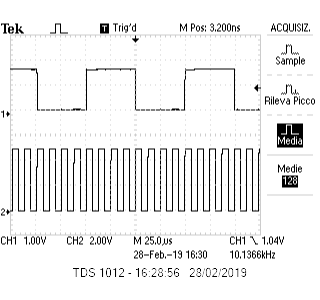
\includegraphics[width=\linewidth]{immagini/f1_8}
		\captionof{figure}{$Q_2$}
		\label{fig:f1_8}
	\end{minipage}
	\begin{minipage}{.5\linewidth}
		\centering
		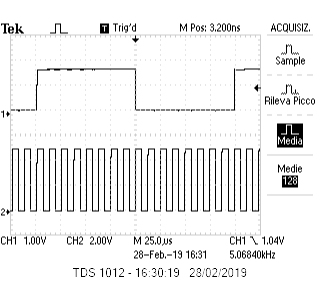
\includegraphics[width=\linewidth]{immagini/f1_16}
		\captionof{figure}{$Q_3$}
		\label{fig:f1_16}
	\end{minipage}\newline
	Essendo un contatore sincrono gli i tempi di sfasamento delle varie uscite sono uguali tra di loro. Il tempo di sfasamento da LOW a HIGH è $t_{LH}=27.3\pm0.9ns$ e $t_{HL}=63\pm1ns$. La stima degli errori è stata effettuata considerando il valore massimo e quello minimo notabile dello sfasamento e facendo la media e la somma dimezzata. (non so spiegarlo decentemente lorenzo aiuto!)\newline
	Purtroppo ci siamo dimenticati ad acquisire le immagini dell'acquisizione dall'oscilloscopio.\newline
	\subparagraph{d)Contatore decimale}
		Quando il contatore arriva a 9 si ha che $(Q_0,Q_1,Q_2,Q_3)=(1,0,0,1)$, in particolare esso è il primo numero che ha sia la porta $Q_0$ e $Q_3$ HIGH, quindi può essere usata come condizione per resettare il contatore. Essendo di defaut la porta di RESET HIGH basta collegare al RESET un NAND che ha come ingressi $Q_0$ e $Q_3$.\newline
		Le immagini dell'output dell'oscilloscopio sono visibili nell'immagine \ref{fig:3d}
		\begin{figure}
		\begin{center}
			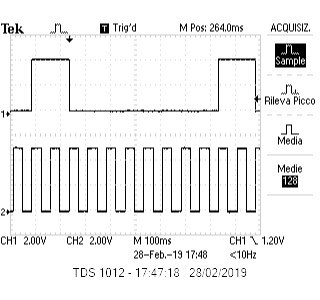
\includegraphics[width=0.5\linewidth]{immagini/3d}
			\captionof{figure}{Contatore decimale}
			\label{fig:3d}
		\end{center}
		\end{figure}
\end{document}